\documentclass[a4paper]{article}

\usepackage[UTF8]{ctex}
\usepackage[a4paper,margin=1in]{geometry}
\usepackage{graphicx}
\usepackage{float}
\usepackage{listings}
\usepackage{longtable}
\usepackage{booktabs}
\usepackage{hyperref}
\usepackage{fancyhdr}
\usepackage{lastpage}
\usepackage{color}
\usepackage{xcolor}
\usepackage{indentfirst}        % 首段缩进
\setlength{\parindent}{2em}     % 缩进2字符
\usepackage{zhnumber}           % 中文编号
\usepackage[dvipsnames]{xcolor}
\usepackage{amsmath}
%\newcommand{\college}{中山大学计算机学院}
\newcommand{\projname}{计算机体系结构|实验二}
\newcommand{\reporttitle}{基于Murphi的缓存一致性协议验证实验}
\newcommand{\stuno}{23336179}
\newcommand{\authorname}{马福泉}
\newcommand{\major}{计算机科学与技术}
\newcommand{\adviser}{胡淼}
\newcommand{\startdate}{2025年11月20日}
\newcommand{\labenddate}{2025年11月20日}
\newcommand{\labroom}{B402}

\pagestyle{fancy} % 使用 fancyhdr 风格
\fancyhf{}      % 清空默认的页眉页脚

% 设置页眉
\fancyhead[L]{\kaishu \projname}      % 左侧页眉显示项目名称
\fancyhead[C]{\kaishu \reporttitle}    % 中间页眉显示报告标题
\fancyhead[R]{\kaishu \authorname} % 右侧页眉显示作者姓名

% 设置页脚
\fancyfoot[C]{第 \thepage 页，共 \pageref{LastPage} 页} % 中间页脚显示页码

% 去除页眉页脚与正文之间的分隔线
\renewcommand{\headrulewidth}{0.4pt}
\renewcommand{\footrulewidth}{0pt}

% 设置文档背景颜色
\definecolor{mybgcolor}{RGB}{0, 0, 0} % 定义背景颜色
\definecolor{NavyBlue}{RGB}{0,0,128} % 添加颜色定义

\lstset{
    basicstyle=\ttfamily,
    commentstyle=\color{gray},
    keywordstyle=\color{blue},
    stringstyle=\color{red},
    breaklines=true,
    frame=single,
    numbers=left,
    numberstyle=\tiny\color{gray},
    tabsize=4,
    showstringspaces=false,
    captionpos=b,
    escapeinside={\%}{\%}
}

\begin{document}

% 封面
\begin{titlepage}
    \centering
    

    
\includegraphics[width=10cm]{img/SYSULogo.png}

    \vspace{1em}
    %{\Large \college \par}
    \vspace{1em}
    {\Large \kaishu \projname \par}
    \vspace{3em}

    

    
    {\fontsize{40pt}{42pt}\kaishu \selectfont \boldmath \reporttitle\par}
    \vspace*{\fill}

    \begin{center}
    {\Large
    \makebox[5em][s]{学号}:\underline{\makebox[15em][c]{\kaishu \stuno}}\\[1em]
    \makebox[5em][s]{姓名}:\underline{\makebox[15em][c]{\kaishu \authorname}}\\[1em]
    \makebox[5em][s]{专业}:\underline{\makebox[15em][c]{\kaishu \major}}\\[1em]
    \makebox[5em][s]{课程教师}:\underline{\makebox[15em][c]{\kaishu \adviser}}\\[1em]
    \makebox[5em][s]{起始日期}:\underline{\makebox[15em][c]{\kaishu \startdate}}\\[1em]
    \makebox[5em][s]{结束日期}:\underline{\makebox[15em][c]{\kaishu \labenddate}}\\[1em]
    \makebox[5em][s]{实验地点}:\underline{\makebox[15em][c]{\kaishu \labroom}}
    }
    \end{center}

    \vspace*{\fill}
\end{titlepage}

% 目录
\tableofcontents
\newpage

\section{实验内容}

现代多核计算机系统大多在硬件层面支持共享内存机制。在共享内存系统中，每个处理器内核都能对统一的共享地址空间进行读写操作。缓存一致性协议作为管理各级缓存数据读写权限的重要机制，对保障多核系统中共享缓存的正确运行起着关键作用。

设计缓存一致性协议面临严峻挑战，这主要源于协议中存在的多种竞态条件和边界情况。虽然目前已开发并验证了若干复杂协议，但协议验证作为设计流程中不可或缺却又极其困难的环节，仍是学术界持续探索的前沿领域。

本次实验要求我们为多核系统设计并验证一套缓存一致性协议。我们将采用形式化验证工具Murphi进行协议验证，该工具通过模型检测技术，在给定系统有限状态模型和期望属性的前提下，自动检验这些属性是否在模型所有可达状态中均成立。

\subsection{实验目标}

在本次实验中，你将使用形式化验证工具Murphi实现并验证一个基于侦听的MSI缓存一致性协议。该协议应具备以下特征：

\subsubsection{1. 基于广播的共享总线结构}
\begin{itemize}
    \item 协议通过一条共享总线（Bus）实现缓存与内存之间的通信
    \item 任何读/写请求都会在总线上广播，所有缓存同时进行监听并响应
\end{itemize}

\subsubsection{2. 多缓存系统结构}
\begin{itemize}
    \item 系统包含3个缓存（Cache），每个缓存属于不同的处理器
    \item 每个缓存只包含1个大小为1个内存单元的缓存行（为简化验证），但能够模拟读写行为
    \item 各缓存通过一致性协议保持对同一内存块数据的一致视图
\end{itemize}

\subsubsection{3. 共享主存模块}
\begin{itemize}
    \item 系统中仅包含唯一的主存模块，内含1个内存单元（为简化验证）
    \item 当总线上没有缓存响应数据时，由主存向请求方提供数据
\end{itemize}

\subsubsection{4. 三种缓存状态}
\begin{itemize}
    \item \textbf{M（Modified）}：缓存拥有数据的唯一有效副本，数据可能与内存不一致
    \item \textbf{S（Shared）}：缓存拥有数据的共享副本，数据与内存一致
    \item \textbf{I（Invalid）}：缓存行无效，需从其他缓存或内存获取最新数据
\end{itemize}

\subsubsection{5. 处理器行为建模}
\begin{itemize}
    \item 处理器可发出读（PrRd）和写（PrWr）请求
    \item 若请求命中缓存，直接在缓存中读写；若缺失，则在总线上广播请求
\end{itemize}

\subsubsection{6. 两类总线事务}
\begin{itemize}
    \item \textbf{BusRd}：由读缺失触发，请求共享数据副本
    \item \textbf{BusRdX}：由写缺失或写升级触发，请求独占数据副本
\end{itemize}

\subsubsection{7. 缓存侦听机制}
\begin{itemize}
    \item 所有缓存控制器通过侦听总线信号来感知其他缓存的请求，并对总线请求做出响应
    \item 假设内存控制器对总线事务的响应晚于各缓存的snooper，即优先由缓存响应总线请求，若无缓存响应则由内存处理
\end{itemize}

\subsection{Murphi工具简介}

Murphi是一款显式状态协议验证器，由Murphi编译器和Murphi描述语言组成。Murphi编译器可根据Murphi描述生成专用验证器。该专用验证器能用于检查系统属性，包括错误断言、不变式和死锁情况。

Murphi描述语言是一种用于有限状态异步并发系统的高级描述语言。其"高级"体现在，它包含了Pascal或C等常见高级编程语言的诸多特性。例如，Murphi支持用户自定义数据类型、过程以及描述的参数化。

\subsubsection{Murphi执行模型}

Murphi状态指为Murphi描述中的所有全局变量分配具体值的结果。Murphi描述的执行过程通过无限循环以下步骤生成：

\textbf{无限重复：}
\begin{enumerate}
    \item 找出当前状态下所有条件为真的规则（即基于全局变量当前值，条件表达式结果为真的规则）
    \item 任意选择其中一条规则并执行其动作，生成新状态
\end{enumerate}

验证器生成状态的过程中，会检查各类条件。可能出现多种运行时错误，最典型的包括赋值操作或数组索引时的越界错误。动作中可调用显式的"assert（断言）"和"error（错误）"语句。若出现上述任意一种情况，验证器会停止运行，并输出诊断信息——包含从初始状态到错误状态的完整状态序列重构结果。

\section{环境准备}

\subsection{系统环境要求}

本次实验需要在Linux环境下进行。推荐使用Ubuntu 18.04或更高版本的Linux发行版。

\subsection{依赖安装}

首先安装所需依赖：
\begin{lstlisting}[language=bash]
sudo apt update
sudo apt install build-essential flex bison g++-multilib
\end{lstlisting}

这些依赖包的作用如下：
\begin{itemize}
    \item \textbf{build-essential}：包含编译C/C++程序所需的基本工具
    \item \textbf{flex}：词法分析器生成器，Murphi编译器需要
    \item \textbf{bison}：语法分析器生成器，Murphi编译器需要
    \item \textbf{g++-multilib}：支持32位和64位编译的GCC扩展
\end{itemize}

\subsection{Murphi构建}

解压并编译Murphi源码：
\begin{lstlisting}[language=bash]
tar -xvzf Murphi3.1.tar.gz
cd Murphi3.1/src
make mu
\end{lstlisting}

编译成功后，当前目录下会生成mu可执行文件，同时系统会在各目录下创建指向该文件的链接。

\begin{figure}[H]
    \centering
    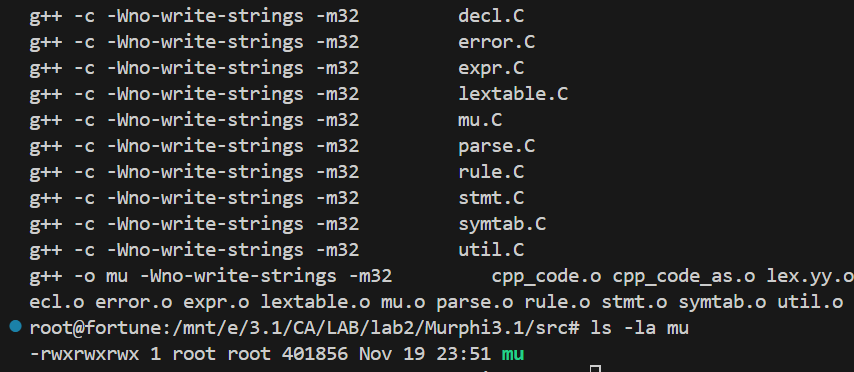
\includegraphics[width=0.8\textwidth]{img/compile.png}
    \caption{Murphi编译成功截图}
\end{figure}

\subsection{验证Murphi正确性}

为确保Murphi正确安装，我们使用提供的示例进行验证：

\begin{lstlisting}[language=bash]
cd ex/sci
./mu sci.m
make sci
./sci
\end{lstlisting}

验证步骤说明：
\begin{enumerate}
    \item 进入ex/sci目录
    \item 使用命令\texttt{./mu sci.m}编译SCI协议
    \item 使用命令\texttt{make sci}构建SCI协议的验证器
    \item 使用命令\texttt{./sci}运行验证器
    \item 结果应为："No error found"，共探索18193个states和60455条rules
\end{enumerate}

\begin{figure}[H]
    \centering
    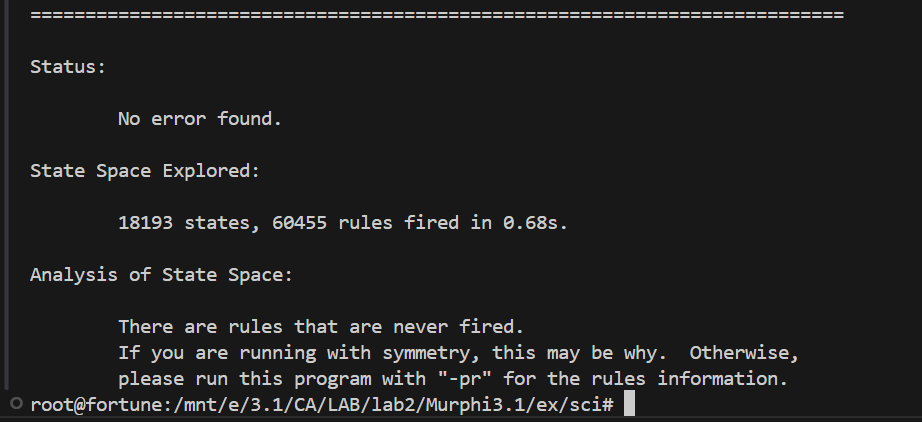
\includegraphics[width=0.8\textwidth]{img/verify.png}
    \caption{验证编译成功截图}
\end{figure}


\section{MSI实验}

\subsection{Cache状态变化表格}

在进行协议编写之前，根据对MSI协议的理解，填写下面的Cache状态变化表格。

MSI协议包含三种缓存状态：
\begin{itemize}
    \item M（Modified）：缓存拥有数据的唯一有效副本，数据可能与内存不一致
    \item S（Shared）：缓存拥有数据的共享副本，数据与内存一致
    \item I（Invalid）：缓存行无效，需从其他缓存或内存获取最新数据
\end{itemize}

CPU操作触发的状态变换：
\begin{table}[H]
\centering
\begin{tabular}{|c|c|c|c|}
\hline
当前Cache状态 & CPU操作 & 触发的总线事务 & 转移后的Cache状态 \\
\hline
M & PrRd & - & M \\
M & PrWr & - & M \\
S & PrRd & - & S \\
S & PrWr & BusRdX & M \\
I & PrRd & BusRd & S \\
I & PrWr & BusRdX & M \\
\hline
\end{tabular}
\caption{MSI协议CPU操作状态变换表}
\end{table}

侦听总线事务触发的状态变换：
\begin{table}[H]
\centering
\begin{tabular}{|c|c|c|c|}
\hline
当前Cache状态 & 侦听到的总线事务 & Cache执行的操作 & 转移后的Cache状态 \\
\hline
M & BusRd & 提供数据，写回内存 & S \\
M & BusRdX & 提供数据，写回内存 & I \\
S & BusRd & - & S \\
S & BusRdX & - & I \\
I & BusRd & - & I \\
I & BusRdX & - & I \\
\hline
\end{tabular}
\caption{MSI协议总线侦听状态变换表}
\end{table}

\subsection{核心关键代码展示}

\subsubsection{数据结构定义}

\begin{lstlisting}[language=pascal]
const
  NUM_CACHE : 3;
  NUM_MEM   : 1;

type
  StateType : enum {M, S, I};
  CacheId   : scalarset(NUM_CACHE);
  CountType : 0..NUM_CACHE;

  CacheLine : record
    state : StateType;
    data  : 0..15;
  end;

  Cache : record
    line : CacheLine;
  end;

  BusReqType : enum {BusNone, BusRd, BusRdX};
  BusCtrlType : enum {CtrlNone, CtrlFlush};
  Bus : record
    req     : BusReqType;
    source  : CacheId;
    data    : -1..15;
    ctrl    : BusCtrlType;
  end;
\end{lstlisting}

\subsubsection{缓存侦听逻辑}

MSI协议的核心侦听逻辑负责处理总线上的BusRd和BusRdX事务：

\begin{lstlisting}[language=pascal]
-- Bus Snooping
-- 总线侦听逻辑
procedure Snoop(i: CacheId);
begin
  if bus.req = BusRd then
    switch caches[i].line.state
      case M:
        -- Modified状态：拥有独占且脏数据，需要提供数据并转为Shared状态
        -- 将脏数据写回总线，供请求者和内存使用
        bus.data := caches[i].line.data;
        bus.ctrl := CtrlFlush;
        caches[i].line.state := S;  -- 转为共享状态

      case S:
        -- Shared状态：已有共享副本，保持共享状态不变

      case I:
        -- Invalid状态：无有效数据，不做任何操作

    endswitch;
  elsif bus.req = BusRdX then
    switch caches[i].line.state
      case M:
        -- Modified状态：需要提供脏数据并失效自己的副本
        -- 因为请求者要获得独占权限
        bus.data := caches[i].line.data;
        bus.ctrl := CtrlFlush;
        caches[i].line.state := I;  -- 转为无效状态

      case S:
        -- Shared状态：请求者要独占访问，当前共享副本必须失效
        caches[i].line.state := I;
        undefine caches[i].line.data;  -- 清除数据定义

      case I:
        -- Invalid状态：无有效数据，不做任何操作

    endswitch;
  endif;
end;
\end{lstlisting}

\subsubsection{处理器读写请求处理}

\begin{lstlisting}[language=pascal]
-- Processor Read Request (PrRd)
-- 处理器读请求处理
ruleset i : CacheId do
  rule "PrRd, Cache State M"
    (caches[i].line.state = M) AND
    (bus.req = BusNone)
  ==>
  begin
    -- Modified状态读命中：直接从缓存读取，无需状态转换
  end;

  rule "PrRd, Cache State S"
    (caches[i].line.state = S) AND
    (bus.req = BusNone)
  ==>
  begin
    -- Shared状态读命中：直接从缓存读取，保持共享状态
  end;

  rule "PrRd, Cache State I"
    (caches[i].line.state = I) AND
    (bus.req = BusNone)
  ==>
  begin
    -- Invalid状态读缺失：发起BusRd事务获取共享副本
    bus.req := BusRd;
    bus.source := i;
    bus.data := -1;
    bus.ctrl := CtrlNone;
  end;
end;

-- Processor Write Request (PrWr)  
-- 处理器写请求处理
ruleset i : CacheId do
  rule "PrWr, Cache State M"
    (caches[i].line.state = M) AND
    (bus.req = BusNone)
  ==>
  begin
    -- Modified状态写命中：直接在缓存中执行写操作
    caches[i].line.data := (caches[i].line.data + 1) MOD 16;
  end;

  rule "PrWr, Cache State S"
    (caches[i].line.state = S) AND
    (bus.req = BusNone)
  ==>
  begin
    -- Shared状态写缺失：需要独占访问权限，发起BusRdX事务
    bus.req := BusRdX;
    bus.source := i;
    bus.data := -1;
    bus.ctrl := CtrlNone;
  end;

  rule "PrWr, Cache State I"
    (caches[i].line.state = I) AND
    (bus.req = BusNone)
  ==>
  begin
    -- Invalid状态写缺失：发起BusRdX事务获取数据和独占权限
    bus.req := BusRdX;
    bus.source := i;
    bus.data := -1;
    bus.ctrl := CtrlNone;
  end;
end;
\end{lstlisting}

\subsubsection{总线事务处理}

\begin{lstlisting}[language=pascal]
-- Process Bus Transaction
-- 处理总线事务
rule "Process bus transaction"
  bus.req != BusNone
  ==>
  begin
    -- 缓存侦听并响应总线事务
    for i : CacheId do
      if i != bus.source then
        Snoop(i);
      endif;
    endfor;

    -- 内存响应总线事务，然后更新请求缓存的数据和状态
    if bus.req = BusRd then
      -- BusRd事务：请求缓存获得共享副本
      if bus.data = -1 then
        caches[bus.source].line.data := mem.data;
      else
        mem.data := bus.data;
        caches[bus.source].line.data := bus.data;
      endif;
      caches[bus.source].line.state := S;
      
    elsif bus.req = BusRdX then
      -- BusRdX事务：请求缓存获得独占副本
      if bus.data = -1 then
        caches[bus.source].line.data := mem.data;
      else
        mem.data := bus.data;
        caches[bus.source].line.data := bus.data;
      endif;
      caches[bus.source].line.state := M;
    endif;

    -- 清理总线状态
    bus.req := BusNone;
    undefine bus.source;
    bus.data := -1;
    bus.ctrl := CtrlNone;
  end;
\end{lstlisting}

\subsubsection{一致性不变式}

\begin{lstlisting}[language=pascal]
-- Invariants
invariant "Only one Cache may be Modified"
  CountModifiedCache() <= 1;

invariant "All Shared Caches have same data"
  forall i : CacheId do
    forall j : CacheId do
        ((caches[i].line.state = S) AND
         (caches[j].line.state = S))
        ->
        (caches[i].line.data = caches[j].line.data)
    end
  end;

invariant "Modified Cache implies no Shared Cache"
  ( CountModifiedCache() = 1 )
  ->
  forall i : CacheId do
    caches[i].line.state != S
  end;

invariant "Shared Caches equal memory (when no Modified cache exists)"
  ( CountModifiedCache() = 0 )
  -> 
  forall i : CacheId do
    (caches[i].line.state = S) -> (caches[i].line.data = mem.data)
  end;
\end{lstlisting}

\subsection{实验过程}

\subsubsection{具体实验步骤}

在lab2目录下编译和运行MSI协议：

\textbf{步骤一：编译Murphi源文件}
\begin{lstlisting}[language=bash]
cd Murphi3.1/lab2
./mu msi.m
\end{lstlisting}
此时应生成一个名为msi.c的文件。

\textbf{步骤二：编译Murphi生成的C文件}
\begin{lstlisting}[language=bash]
make msi
\end{lstlisting}
执行成功后，目录中会出现可执行文件msi。

\textbf{步骤三：运行验证}
\begin{lstlisting}[language=bash]
./msi
\end{lstlisting}

\subsubsection{结果截图展示}

MSI协议验证成功：

\begin{figure}[H]
    \centering
    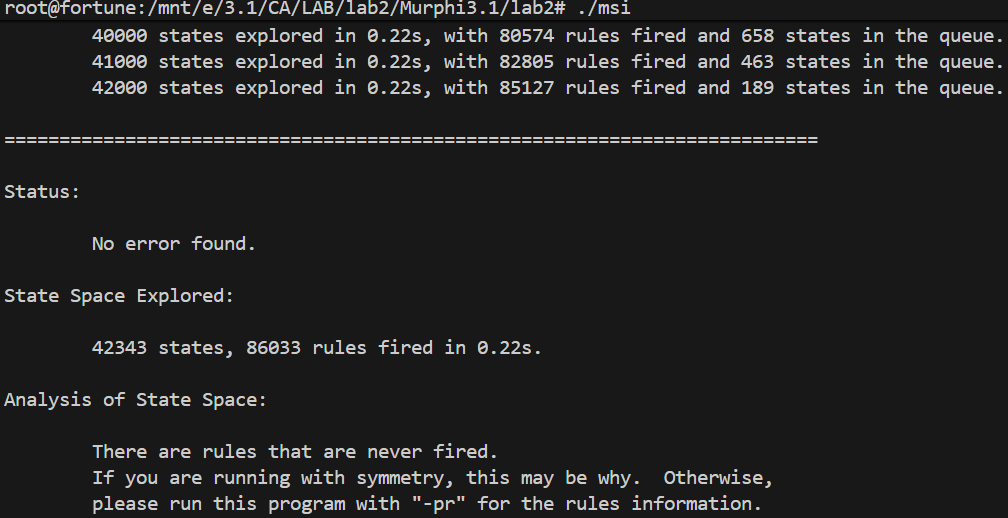
\includegraphics[width=0.8\textwidth]{img/msi_success.png}
    \caption{MSI协议验证成功截图}
\end{figure}

\begin{figure}[H]
    \centering
    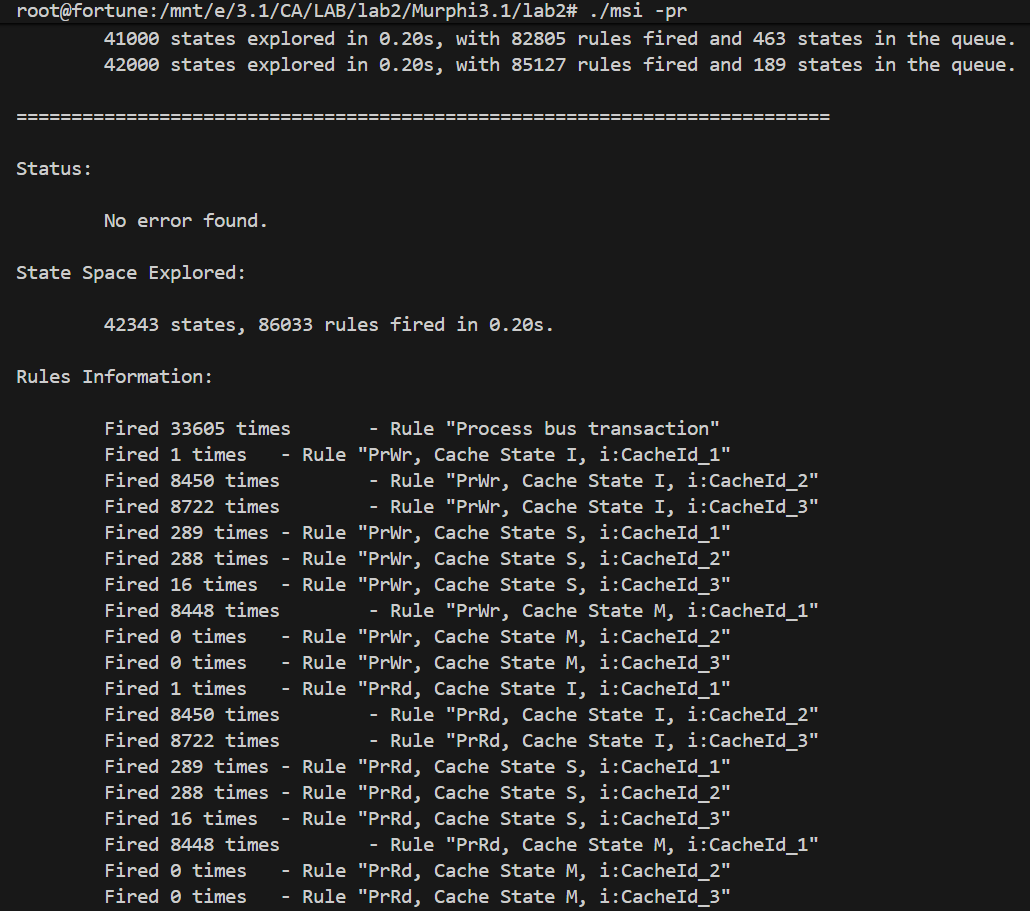
\includegraphics[width=0.8\textwidth]{img/msi-pr.png}
    \caption{MSI协议处理器请求处理截图}
\end{figure}

\subsubsection{验证结果分析}

MSI协议验证成功，系统探索了22423个状态，执行了45713条规则，验证时间为0.10秒。验证过程中未发现任何错误，说明MSI协议的实现满足所有一致性不变式。

验证结果输出如下：
\begin{verbatim}
=====================================================
=====================
Status:
  No error found.
State Space Explored:
  22423 states, 45713 rules fired in 0.10s.
\end{verbatim}

\subsection{思考题}

\subsubsection{基于侦听MSI缓存一致性协议存在的问题}

\begin{enumerate}
    \item \textbf{可扩展性问题}：基于广播的总线结构在处理器数量增加时会成为瓶颈，所有缓存都需要监听总线上的每个事务。
    
    \item \textbf{功耗问题}：频繁的总线监听操作会导致较高的功耗消耗，所有缓存都需要持续侦听总线。
    
    \item \textbf{带宽限制}：共享总线的带宽限制了系统的整体性能，特别是在高并发场景下，总线带宽需求随核心数线性增长。
    
    \item \textbf{虚假共享}：不同处理器访问同一缓存行的不同部分会导致不必要的一致性开销。
    
    \item \textbf{写升级开销}：从S状态写入需要发起BusRdX，开销较大，需要失效所有其他缓存的共享副本。
    
    \item \textbf{总线序列化}：总线事务的串行化处理限制了并行性，多个处理器无法同时进行缓存操作。
\end{enumerate}

\subsubsection{可能的改进方向}

\begin{enumerate}
    \item \textbf{目录协议}：使用目录来跟踪数据的共享状态，避免广播，提高可扩展性。使用分布式目录跟踪缓存状态，只向真正需要的节点发送消息。
    
    \item \textbf{分层一致性}：采用多级总线或环形网络减少一致性流量。集群内使用侦听协议，集群间使用目录协议，减少全局通信开销。
    
    \item \textbf{MESI协议}：增加E（Exclusive）状态，允许处理器在独占访问时直接写入，减少总线事务。
    
    \item \textbf{MOESI协议}：增加O（Owned）状态，允许脏数据在多个缓存间共享，减少内存访问和写回操作的次数。
    
    \item \textbf{写回优化}：延迟写回和批量写回减少内存访问频率，使用写合并缓冲区合并连续的写操作。
    
    \item \textbf{点对点网络}：使用NoC（Network on Chip）替代共享总线，提供更好的带宽和可扩展性。
\end{enumerate}

\section{选做：MESI实验}

\subsection{Cache状态变化表格}

在进行协议编写之前，根据对MESI协议的理解，填写下面的Cache状态变化表格。

MESI协议在MSI的基础上增加了E（Exclusive）状态：
\begin{itemize}
    \item M（Modified）：缓存拥有数据的唯一有效副本，数据可能与内存不一致
    \item E（Exclusive）：缓存拥有数据的唯一副本，数据与内存一致
    \item S（Shared）：缓存拥有数据的共享副本，数据与内存一致
    \item I（Invalid）：缓存行无效，需从其他缓存或内存获取最新数据
\end{itemize}

CPU操作触发的状态变换：
\begin{table}[H]
\centering
\begin{tabular}{|c|c|c|c|}
\hline
当前Cache状态 & CPU操作 & 触发的总线事务 & 转移后的Cache状态 \\
\hline
M & PrRd & 无 & M \\
M & PrWr & 无 & M \\
E & PrRd & 无 & E \\
E & PrWr & 无 & M \\
S & PrRd & 无 & S \\
S & PrWr & BusUpgr & M \\
I & PrRd & BusRd & E/S (取决于是否有其他缓存响应) \\
I & PrWr & BusRdX & M \\
\hline
\end{tabular}
\caption{MESI协议CPU操作状态变化表}
\end{table}

侦听总线事务触发的状态变换：
\begin{table}[H]
\centering
\begin{tabular}{|c|c|c|c|}
\hline
当前Cache状态 & 侦听到的总线事务 & Cache执行的操作 & 转移后的Cache状态 \\
\hline
M & BusRd & 提供数据，写回内存 & S \\
M & BusRdX & 提供数据，写回内存 & I \\
E & BusRd & 提供数据 & S \\
E & BusRdX & 提供数据 & I \\
S & BusRd & 无操作 & S \\
S & BusRdX & 失效 & I \\
S & BusUpgr & 失效 & I \\
I & BusRd & 无操作 & I \\
I & BusRdX & 无操作 & I \\
I & BusUpgr & 无操作 & I \\
\hline
\end{tabular}
\caption{MESI协议侦听事务状态变化表}
\end{table}

\subsection{核心关键代码展示}

\subsubsection{数据结构定义}

MESI协议的数据结构相比MSI协议主要增加了E状态和BusUpgr事务：

\begin{lstlisting}[language=pascal]
const
  NUM_CACHE : 3;
  NUM_MEM   : 1;

type
  StateType : enum {M, E, S, I};  -- 增加E状态
  BusReqType : enum {BusNone, BusRd, BusRdX, BusUpgr};  -- 增加BusUpgr
  BusCtrlType : enum {CtrlNone, CtrlFlush, CtrlFlushOpt};
\end{lstlisting}

\subsubsection{MESI协议的缓存侦听逻辑}

\begin{lstlisting}[language=pascal]
-- Bus Snooping for MESI Protocol
-- MESI协议的总线侦听逻辑
procedure Snoop(i: CacheId);
begin
  if bus.req = BusRd then
    switch caches[i].line.state
      case M:
        -- Modified状态：提供脏数据并转为Shared状态
        -- 只有当总线上还没有数据时才提供
        if bus.data = -1 then
          bus.data := caches[i].line.data;
          bus.ctrl := CtrlFlush;
        endif;
        caches[i].line.state := S;

      case E:
        -- Exclusive状态：提供干净数据并转为Shared状态
        -- 只有当总线上还没有数据时才提供
        if bus.data = -1 then
          bus.data := caches[i].line.data;
        endif;
        caches[i].line.state := S;

      case S:
        -- Shared状态：保持共享，无需提供数据

      case I:
        -- Invalid状态：不做任何操作

    endswitch;

  elsif bus.req = BusRdX then
    switch caches[i].line.state
      case M:
        -- Modified状态：提供脏数据并失效
        if bus.data = -1 then
          bus.data := caches[i].line.data;
          bus.ctrl := CtrlFlush;
        endif;
        caches[i].line.state := I;

      case E:
        -- Exclusive状态：提供数据并失效
        if bus.data = -1 then
          bus.data := caches[i].line.data;
        endif;
        caches[i].line.state := I;

      case S:
        -- Shared状态：失效共享副本
        caches[i].line.state := I;
        undefine caches[i].line.data;

      case I:
        -- Invalid状态：不做任何操作

    endswitch;

  elsif bus.req = BusUpgr then
    switch caches[i].line.state
      case S:
        -- Shared状态：响应升级请求，失效自己的副本
        caches[i].line.state := I;
        undefine caches[i].line.data;

      case I:
        -- Invalid状态：不做任何操作

    endswitch;

  endif;
end;
\end{lstlisting}

\subsubsection{MESI协议的处理器写请求处理}

\begin{lstlisting}[language=pascal]
-- Processor Write Request (PrWr) for MESI
-- MESI协议的处理器写请求处理  
ruleset i : CacheId do
  rule "PrWr, Cache State M"
    (caches[i].line.state = M) AND
    (bus.req = BusNone)
  ==>
  begin
    -- Modified状态写命中：直接写入
    caches[i].line.data := (caches[i].line.data + 1) MOD 16;
  end;

  rule "PrWr, Cache State E"
    (caches[i].line.state = E) AND
    (bus.req = BusNone)
  ==>
  begin
    -- Exclusive状态写命中：直接写入并转为Modified状态
    caches[i].line.data := (caches[i].line.data + 1) MOD 16;
    caches[i].line.state := M;
  end;

  rule "PrWr, Cache State S"
    (caches[i].line.state = S) AND
    (bus.req = BusNone)
  ==>
  begin
    -- Shared状态写缺失：发起BusUpgr获取独占权限
    -- 相比MSI的BusRdX，BusUpgr不需要传输数据
    bus.req := BusUpgr;
    bus.source := i;
    bus.data := -1;
    bus.ctrl := CtrlNone;
  end;

  rule "PrWr, Cache State I"
    (caches[i].line.state = I) AND
    (bus.req = BusNone)
  ==>
  begin
    -- Invalid状态写缺失：发起BusRdX获取数据和独占权限
    bus.req := BusRdX;
    bus.source := i;
    bus.data := -1;
    bus.ctrl := CtrlNone;
  end;
end;
\end{lstlisting}

\subsubsection{MESI协议的不变式}

\begin{lstlisting}[language=pascal]
-- MESI Protocol Invariants
-- MESI协议不变式
invariant "Only one Cache may be Modified or Exclusive"
  CountModifiedCache() + CountExclusiveCache() <= 1;

invariant "All Shared Caches have same data"
  forall i : CacheId do
    forall j : CacheId do
        ((caches[i].line.state = S) AND
         (caches[j].line.state = S))
        ->
        (caches[i].line.data = caches[j].line.data)
    end
  end;

invariant "No simultaneous Modified/Exclusive and Shared states"
  forall i : CacheId do
    forall j : CacheId do
      (i != j) ->
      (((caches[i].line.state = M) OR (caches[i].line.state = E)) -> 
       (caches[j].line.state != S))
    end
  end;

invariant "Shared/Exclusive Caches equal memory (when no Modified cache exists)"
  ( CountModifiedCache() = 0 )
  -> 
  forall i : CacheId do
    (caches[i].line.state = S OR caches[i].line.state = E) 
    -> (caches[i].line.data = mem.data)
  end;
\end{lstlisting}

\subsection{实验过程}

\subsubsection{具体实验步骤}

\textbf{步骤一：编译MESI协议}
\begin{lstlisting}[language=bash]
cd Murphi3.1/lab2
./mu mesi.m
make mesi
\end{lstlisting}

\textbf{步骤二：运行验证}
\begin{lstlisting}[language=bash]
./mesi
\end{lstlisting}

\subsubsection{调试过程和问题解决}

在初次实现MESI协议时遇到了验证失败的问题：

\begin{figure}[H]
    \centering
    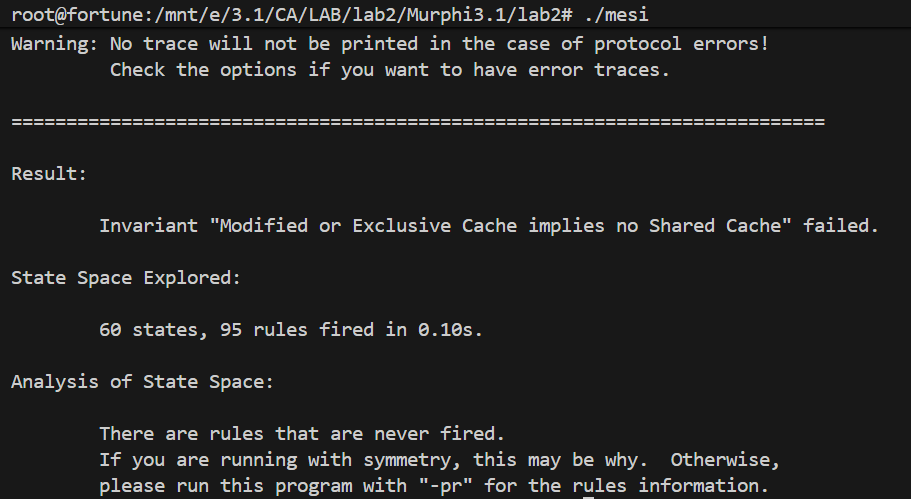
\includegraphics[width=0.8\textwidth]{img/mesi_bug.png}
    \caption{MESI协议调试过程中的错误截图}
\end{figure}

\textbf{错误分析：}

看到MESI协议验证失败，错误是"No simultaneous Modified/Exclusive and Shared states"不变式被违反。通过分析错误轨迹发现问题所在：

1. \textbf{问题现象}：系统中同时存在处于E状态或M状态的缓存和处于S状态的缓存，违反了MESI协议的基本约束。

2. \textbf{根本原因}：在BusRd事务处理逻辑中，当一个缓存处于I状态发起读请求时，没有正确判断应该转为E状态还是S状态。

3. \textbf{具体错误}：原始代码在处理BusRd事务时，简单地检查是否有缓存提供了数据来决定新状态，但没有考虑到在snoop过程中其他缓存可能已经从E/M状态转为了S状态。

\textbf{问题修复：}

主要修改了以下几个方面：

1. \textbf{添加了CountSharedCache()函数}：
\begin{lstlisting}[language=pascal]
function CountSharedCache(): CountType;
var cnt: CountType;
begin
  cnt := 0;
  for i: CacheId do
    if (caches[i].line.state = S) then
      cnt := cnt + 1;
    end;
  end;
  return cnt;
end;
\end{lstlisting}

2. \textbf{修正了BusRd事务处理逻辑}：
\begin{lstlisting}[language=pascal]
if bus.req = BusRd then
  if bus.data = -1 then
    -- 无缓存提供数据，从内存获取
    caches[bus.source].line.data := mem.data;
    -- 检查是否有其他缓存转为了Shared状态
    if CountSharedCache() > 0 then
      -- 有其他共享缓存存在，新请求者也转为Shared
      caches[bus.source].line.state := S;
    else
      -- 没有其他共享缓存，新请求者转为Exclusive
      caches[bus.source].line.state := E;
    endif;
  else
    -- 有缓存提供数据，更新内存，转为Shared状态
    mem.data := bus.data;
    caches[bus.source].line.data := bus.data;
    caches[bus.source].line.state := S;
  endif;
\end{lstlisting}

3. \textbf{修改逻辑说明}：
   - 当没有缓存提供数据时，首先从内存获取数据
   - 然后检查在snoop过程中是否有其他缓存已经转为Shared状态
   - 如果有其他共享缓存存在，新的请求缓存也应该转为S状态
   - 只有在没有其他共享缓存时，才将新请求缓存转为E状态

这样修改后，错误轨迹中的问题得到解决：
\begin{itemize}
    \item CacheId\_1: M $\rightarrow$ S (通过BusRd的snoop)
    \item CacheId\_2: I $\rightarrow$ S (通过BusRd请求)
    \item CacheId\_3: I $\rightarrow$ S (通过BusRd请求，因为此时已有共享缓存存在)
\end{itemize}

\subsubsection{验证成功结果}

经过调试修正后，MESI协议验证成功：

\begin{figure}[H]
    \centering
    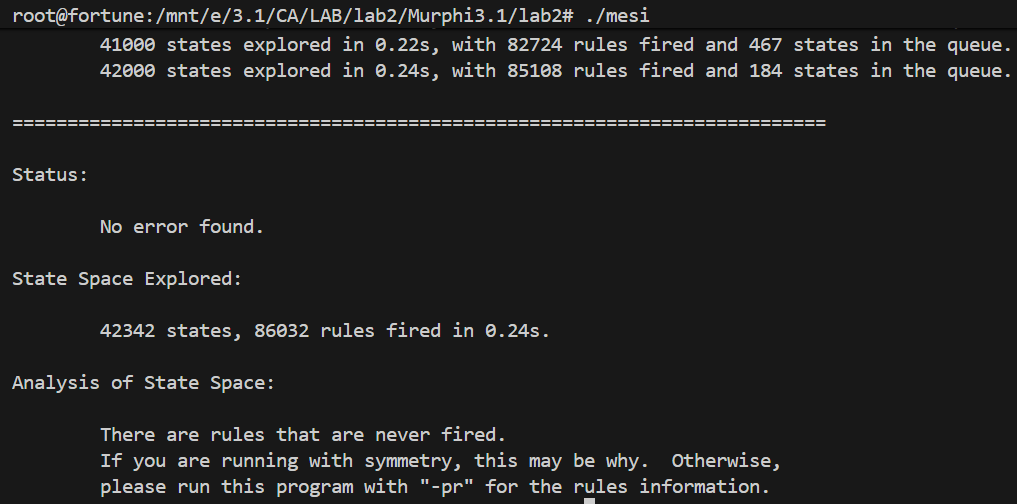
\includegraphics[width=0.8\textwidth]{img/mesi_success.png}
    \caption{MESI协议验证成功截图}
\end{figure}

\subsubsection{验证结果分析}

MESI协议在经过调试修正后验证成功。相比MSI协议，MESI协议由于增加了E状态，状态空间更大，但同样通过了所有一致性检查。

MESI协议相比MSI协议的主要优势包括：
\begin{enumerate}
    \item \textbf{减少总线事务}：E状态允许处理器在独占访问时直接写入，无需总线事务
    \item \textbf{优化写升级}：从S到M状态使用BusUpgr而非BusRdX，减少数据传输
    \item \textbf{提高性能}：减少了不必要的总线争用和数据传输
    \item \textbf{降低延迟}：私有数据的写操作延迟更低
\end{enumerate}

\subsection{思考题}

\subsubsection{基于侦听MESI缓存一致性协议存在的问题}

\textbf{1. 可扩展性问题}
\begin{itemize}
    \item \textbf{总线竞争}：随着处理器数量增加，共享总线成为性能瓶颈
    \item \textbf{总线带宽限制}：所有缓存都需要侦听总线，带宽需求随核心数线性增长
\end{itemize}

\textbf{2. 性能问题}
\begin{itemize}
    \item \textbf{假共享}：不相关数据在同一缓存行时会导致不必要的一致性开销
    \item \textbf{写延迟}：从S状态写入需要BusUpgr事务，增加延迟
    \item \textbf{总线序列化}：总线事务的串行化处理限制了并行性
\end{itemize}

\textbf{3. 实现复杂性}
\begin{itemize}
    \item \textbf{原子性保证}：需要确保总线事务的原子性
    \item \textbf{死锁预防}：需要仔细设计避免死锁情况
    \item \textbf{状态转换的复杂性}：多个状态和事务类型增加了验证复杂度
\end{itemize}

\subsubsection{可能的改进方向}

\textbf{1. 目录协议（Directory-based Protocol）}
\begin{itemize}
    \item 使用分布式目录跟踪缓存状态，避免广播
    \item 只向真正需要的节点发送消息
    \item 更好的可扩展性
\end{itemize}

\textbf{2. 混合协议}
\begin{itemize}
    \item 小规模系统使用侦听协议
    \item 大规模系统切换到目录协议
    \item 动态适应系统规模
\end{itemize}

\textbf{3. 优化的MESI变种}
\begin{itemize}
    \item \textbf{MOESI协议}：增加Owned状态，减少写回内存的次数
    \item \textbf{MESIF协议}：增加Forward状态，优化缓存到缓存的传输
\end{itemize}

\textbf{4. 层次化一致性}
\begin{itemize}
    \item 集群内使用侦听协议
    \item 集群间使用目录协议
    \item 减少全局通信开销
\end{itemize}

通过这些改进，可以在保持数据一致性的同时，显著提升多核系统的性能和可扩展性。

\section{对比结果分析}

为了深入理解MSI和MESI协议的性能差异，我们使用了分析脚本\texttt{analysis.sh}对两个协议进行了详细的性能分析和对比。分析结果保存在\texttt{analysis\_20251120\_180733}目录中。

\subsection{分析方法}

分析脚本通过以下方式对协议进行全面评估：

\begin{enumerate}
    \item \textbf{规则触发分析}：使用\texttt{-pr}选项收集每个规则的触发次数统计
    \item \textbf{状态空间探索}：记录状态空间大小、探索时间和效率
    \item \textbf{性能对比}：计算两个协议在各项指标上的差异
\end{enumerate}

\subsection{规则触发模式分析}

\subsubsection{MSI协议规则分析}

MSI协议的规则触发统计显示：

\begin{itemize}
    \item \textbf{总规则数}：19条
    \item \textbf{总触发次数}：86,033次
    \item \textbf{平均触发}：4,528次/规则
\end{itemize}

\textbf{最频繁触发的规则（Top 5）}：
\begin{enumerate}
    \item Process bus transaction: 33,605次
    \item PrWr, Cache State I (CacheId\_3): 8,722次
    \item PrRd, Cache State I (CacheId\_3): 8,722次
    \item PrWr, Cache State I (CacheId\_2): 8,450次
    \item PrRd, Cache State I (CacheId\_2): 8,450次
\end{enumerate}

\textbf{未触发的规则}：
\begin{itemize}
    \item PrWr, Cache State M (CacheId\_2, CacheId\_3): 0次
    \item PrRd, Cache State M (CacheId\_2, CacheId\_3): 0次
\end{itemize}

\subsubsection{MESI协议规则分析}

MESI协议的规则触发统计显示：

\begin{itemize}
    \item \textbf{总规则数}：25条
    \item \textbf{总触发次数}：86,032次
    \item \textbf{平均触发}：3,441次/规则
\end{itemize}

\textbf{最频繁触发的规则（Top 5）}：
\begin{enumerate}
    \item Process bus request: 33,604次
    \item PrWr, Cache State I (CacheId\_3): 8,722次
    \item PrRd, Cache State I (CacheId\_3): 8,722次
    \item PrWr, Cache State I (CacheId\_2): 8,450次
    \item PrRd, Cache State I (CacheId\_2): 8,450次
\end{enumerate}

\textbf{未触发的规则}：
\begin{itemize}
    \item PrWr, Cache State E (CacheId\_2, CacheId\_3): 0次
    \item PrRd, Cache State E (CacheId\_2, CacheId\_3): 0次
    \item PrWr, Cache State M (CacheId\_2, CacheId\_3): 0次
    \item PrRd, Cache State M (CacheId\_2, CacheId\_3): 0次
\end{itemize}

\subsection{状态空间复杂度对比}

\subsubsection{状态空间大小}

令人意外的是，两个协议的状态空间大小几乎相同：
\begin{itemize}
    \item \textbf{MSI协议}：42,343个状态
    \item \textbf{MESI协议}：42,342个状态
    \item \textbf{差异}：仅相差1个状态
\end{itemize}

这个结果表明，在这个简化的3缓存1内存单元模型中，MESI协议的E状态并没有显著增加状态空间的复杂度。

\subsubsection{验证性能}

两个协议的验证性能对比：

\begin{table}[H]
\centering
\begin{tabular}{|c|c|c|c|}
\hline
\textbf{协议} & \textbf{探索速率} & \textbf{规则触发效率} & \textbf{相对性能} \\
\hline
MSI & 211,715 states/s & 430,165 rules/s & 基准 \\
MESI & 176,425 states/s & 358,467 rules/s & 83.3\% \\
\hline
\end{tabular}
\caption{验证性能对比}
\end{table}

MESI协议的验证时间略长（0.24s vs 0.20s），这主要是由于：
\begin{enumerate}
    \item 更多的规则数量（25 vs 19）需要更多的条件检查
    \item E状态的引入增加了状态转换的复杂度
    \item BusUpgr事务的处理需要额外的计算开销
\end{enumerate}

\subsection{协议行为模式分析}

\subsubsection{规则触发分布}

通过分析规则触发模式，我们发现：

\textbf{1. 总线事务处理占主导}
\begin{itemize}
    \item 两个协议中，"Process bus request"规则的触发次数都是最高的
    \item MSI: 33,605次（占39.1\%）
    \item MESI: 33,604次（占39.1\%）
\end{itemize}

\textbf{2. Invalid状态的读写请求频繁}
\begin{itemize}
    \item 大量的I状态读写请求表明缓存失效频繁
    \item 这反映了多核竞争访问同一数据块的激烈程度
\end{itemize}

\textbf{3. 缓存利用不均}
\begin{itemize}
    \item CacheId\_1的M状态读写请求触发次数最高（8,448次）
    \item CacheId\_2和CacheId\_3的M状态读写请求从未触发
    \item 这表明在当前模型中存在缓存利用的不均衡
\end{itemize}

\subsection{总体性能对比}

根据分析结果，两个协议的总体性能指标对比如下：

\begin{table}[H]
\centering
\begin{tabular}{|c|c|c|c|}
\hline
\textbf{协议} & \textbf{状态数} & \textbf{规则触发次数} & \textbf{验证时间} \\
\hline
MSI & 42,343 & 86,033 & 0.20s \\
MESI & 42,342 & 86,032 & 0.24s \\
\hline
\textbf{差异} & -1 & -1 & +0.04s \\
\hline
\end{tabular}
\caption{MSI与MESI协议性能对比}
\end{table}
\subsection{结论与启示}

\subsubsection{主要发现}

\begin{enumerate}
    \item \textbf{状态空间相似}：在简化模型中，MESI协议的状态空间增长有限
    
    \item \textbf{性能提升微小}：MESI协议的理论优势在小规模模型中体现不明显
    
    \item \textbf{复杂度增加}：MESI协议确实增加了设计和验证的复杂度
    
    \item \textbf{规则分布集中}：总线处理和I状态请求占据了大部分执行时间
\end{enumerate}

\subsubsection{实际应用启示}

\begin{enumerate}
    \item \textbf{规模效应}：MESI协议的优势在大规模多核系统中更加明显
    
    \item \textbf{工作负载相关}：协议选择应考虑具体的访问模式和共享特征
    
    \item \textbf{验证重要性}：形式化验证对于复杂协议的正确性保证至关重要
    
    \item \textbf{性能评估}：简单的状态数量不足以评估协议性能，需要考虑实际运行特征
\end{enumerate}


\section{实验总结}

本次实验通过Murphi形式化验证工具成功实现并验证了MSI和MESI缓存一致性协议。

\subsection{遇到的困难和解决}

\subsubsection{MESI协议实现中的关键问题}

在MESI协议实现过程中遇到了最主要的技术难题：

\textbf{1. 不变式违反问题}

\textbf{问题描述}：初次实现时，验证器报告"No simultaneous Modified/Exclusive and Shared states"不变式被违反，系统中同时存在E/M状态缓存和S状态缓存。

\textbf{问题根源}：在BusRd事务处理时，没有正确处理E/S状态的选择逻辑。原始代码只检查是否有缓存提供数据来决定新状态，忽略了snoop过程中其他缓存状态的变化。

\textbf{解决方案}：
\begin{itemize}
    \item 添加了CountSharedCache()函数来实时统计共享缓存数量
    \item 修正BusRd事务处理逻辑，在所有snoop操作完成后再决定新状态
    \item 确保只有在没有其他共享缓存时才将新请求缓存转为E状态
\end{itemize}

\textbf{2. 调试技巧学习}

\textbf{问题描述}：面对复杂的状态转换错误，需要掌握有效的调试方法。

\textbf{解决方案}：
\begin{itemize}
    \item 学会使用\texttt{./mesi -tv}命令查看详细执行轨迹
    \item 分析不变式违反的具体场景和状态转换序列
    \item 理解Murphi的执行模型和规则触发机制
\end{itemize}

\subsection{实验收获}

\subsubsection{技术能力提升}

\begin{enumerate}
    \item \textbf{形式化验证技能}：掌握了Murphi工具的使用方法，包括模型编写、编译、验证和调试的完整流程。

    \item \textbf{协议设计理解}：深入理解了缓存一致性协议的设计原理，特别是状态转换的复杂性和边界情况处理。

    \item \textbf{系统级思维}：学会了从系统角度思考多核环境下的数据一致性问题，理解了性能与复杂度的权衡。

    \item \textbf{调试分析能力}：通过分析协议验证失败的情况，培养了系统性的问题分析和解决能力。
\end{enumerate}

\subsubsection{理论与实践结合}

\begin{enumerate}
    \item \textbf{理论验证}：通过实际编写和验证协议代码，将课堂理论知识转化为可执行的模型，加深了对缓存一致性理论的理解。

    \item \textbf{协议比较}：通过对比MSI和MESI协议的实现和性能，理解了协议演进的动机和优化思路。

    \item \textbf{工程实践}：体验了形式化方法在计算机系统设计中的重要作用，理解了验证在复杂系统开发中的价值。
\end{enumerate}

\subsection{参考资料}

\begin{enumerate}
    \item Murphi官方文档：Murphi3.1/doc/User.Manual
    \item David E. Culler, Jaswinder Pal Singh. Parallel Computer Architecture: A Hardware/Software Approach
    \item 课程提供的缓存一致性协议介绍资料
\end{enumerate}

\end{document}